\section{Sistemas Embarcados}
\label{sec:embarcados}
Sistemas computacionais fazem parte de diversos produtos desde computadores pessoais e \textit{laptops}, até utensílios domésticos. São conhecidos como sistemas embarcados (SE) os sistemas computacionais que fazem parte de um dispositivo eletrônico maior, não representando sua totalidade, mas oferecendo recursos computacionais específicos para o seu funcionamento \cite{vahid:2002}.

Também pode-se definir um SE como um sistema computacional de propósito específico -- em contraste a um computador pessoal --, que não assume vários papéis de acordo com a necessidade do usuário, apenas realiza tarefas predeterminadas \cite{heath:2002}. Isto é, são sistemas eletrônicos projetados para funções específicas dentro de um dispositivo maior, que pode controlar o meio físico e permite sua interação com o usuário.

Algumas características de sistemas embarcados, segundo \citeonline{schlett:1998}, são restrições específicas, como de custo de produção ou de consumo de energia -- que é o caso de dispositivos móveis, por exemplo, que dependem de uma bateria para funcionar. \citeonline{vahid:2002} citam também como exemplo de sistema embarcado uma câmera fotográfica digital, pois tem um propósito específico (capturar e processar fotografias) e tem restrições de tamanho, custo, e consumo de energia.
%TODO: Consultar \citeonline{vahid:2002}.
\textcolor{red}{TODO!\todo{Falar sobre sistemas de tempo real e descrever as vantagens de sistemas embarcados}}

\subsection{Microcontroladores versus Microprocessadores}
Microcontroladores são processadores com vários componentes integrados, como RAM, uma memória de programa e interfaces de entrada e saída \cite{white:2011}. Os microcontroladores surgiram como um substituto para circuitos lógicos discretos, por serem mais facilmente programáveis e proporcionarem uma funcionalidade maior \cite{heath:2002} e, segundo \citeonline{marwedel:2010}, os processadores em sistemas embarcados são geralmente microcontroladores, por serem simples e fáceis de usar. 
% 
\textcolor{red}{TODO!\todo{Descrever também sobre o preço nos dias atuais.}}

A distinção entre microprocessadores e microcontroladores, contudo, não é tão trivial: \citeonline{schlett:1998} afirma que, de forma simplificada, é comum diferenciá-los tendo como parâmetro seu desempenho, considerando dispositivos de 8 e 16-bit como microcontroladores, e a partir disto como microprocessadores. Mas também existem outros critérios a se considerar, como seu uso e suas possíveis restrições de energia, ou a necessidade de integração com vários componentes periféricos.
\textcolor{red}{TODO!\todo{Apresentar a uma definição de microprocessadores e então detalhar mais as diferenças, bem como, apresentar alguns exemplos com suas especificações.}}

\subsection{IoT: Internet das Coisas}
Com a constante evolução e a ubiquidade da Internet, começam a surgir objetos conectados, transformando dispositivos que já faziam parte do cotidiano em algo que possa ser autônomo e inteligente \cite{kopetz:2011}.  Segundo \citeonline{xia:2012}, o termo ``Internet das Coisas''  não refere-se apenas à existência destes dispositivos inteligentes, mas à interconexão dos objetos do cotidiano através de sistemas embarcados, proporcionando assim ambientes em que os dispositivos se comunicam entre si e também com seres humanos. 
\textcolor{red}{TODO!\todo{Apresentar mais detalhes, bem como, exemplos e contextos de seu uso.}}



\section{Robótica e suas Aplicações}
\label{sec:robotica}
A robótica é uma área que busca sintetizar atividades humanas através do uso de mecanismos, sensores, atuadores e computadores. É comum que pesquisas neste campo seja feita por pesquisadores de outras áreas, servindo como meio para diversos fins \cite{craig:2005}. Sistemas embarcados são tradicionalmente usados na área da robótica, relacionando-se aos aspectos mecânicos \cite{marwedel:2010}. \citeonline{craig:2005} divide a robótica em quatro grandes áreas: manipulação mecânica, locomoção, visão computacional e inteligência artificial.

\subsection{Próteses Robóticas}
\todo[inline,color=lightgray]{Uma aplicação da robótica seria na construção de próteses etc.}
\todo[inline]{Faltando aqui ainda}


\section{Eletromiografia: Geração de Dados}
\label{sec:emg}
A eletromiografia (EMG) é uma técnica que consiste em monitorar atividade neuromuscular, sendo possível assim detectar os potenciais de ação através desta leitura \cite{deluca:1979}. Em teoria, isto significa que, a partir do eletromiograma, é possível identificar a intenção de uma pessoa ao realizar uma atividade motora.

A leitura dos sinais eletromiográficos pode ser feita de diferentes formas: por profundidade ou por superfície. O primeiro método consiste em inserir uma agulha que atinja o músculo desejado, permitindo a captação dos sinais; já a eletromiografia por superfície (sEMG) utiliza apenas um conjunto eletrodos sobre a pele, na região do músculo desejado \cite{deluca:1979}

Com os dados extraídos a partir da EMG, é possível que se desenvolva próteses controláveis baseadas no reconhecimento de padrões e classificação dos dados eletromiográficos dos músculos intactos \cite{park:1998}.
\textcolor{red}{TODO!\todo{Apresentar um exemplo gráfico e descrever como os eletrodos são utilizados, apresentar exemplos de saída e quais os desafios para o reconhecimento de padrões.}}

%TODO: INCLUIR SELEÇÃO DE ATRIBUTOS?


\section{Reconhecimento de Padrões}
\label{sec:patternrec}
O reconhecimento de padrões é um campo que busca encontrar padrões em conjuntos de dados, com finalidade em diversas áreas, e vem sendo desenvolvido ao lado de Aprendizado de Máquina no decorrer dos anos. Com isto, a intenção é usar algoritmos computacionais no intuito de descobrir automaticamente regularidades em dados, possibilitando, por exemplo, a classificação de tais dados \cite{bishop:2006}.

Os dados eletromiográficos podem ser usados para classificação a partir do reconhecimento de padrões. Esta seção abordará o aprendizado de máquina e os algoritmos envolvidos na classificação dos movimentos a partir dos dados dos sensores.
\subsection{Pré-processamento}
\todo[inline,color=lightgray]{Não faço ideia do que colocar nessa seção.}
\todo[inline]{Filtros ou fusão de dados... Depende do sensor a ser utilizado!}%TODO

\subsection{Aprendizado de máquina}
O aprendizado de máquina é importante quando não é possível determinar todos cenários possíveis de um sistema previamente, ou quando se deseja que este se adapte ao ambiente por conta própria \cite{russell:2010}. %TODO
\todo[inline,color=lightgray]{Supervisionada e não supervisionada, utilidade, classificação etc.}

%\subsubsection{Árvores de decisão} %Acho que não é mais necessário

\subsubsection{SVM}
Máquina de Vetores de Suporte (SVM) é uma das técnicas mais populares de aprendizado de máquina supervisionado, por não exigir um conhecimento prévio do domínio em que será aplicado \cite{russell:2010}.

A SVM funciona ao encontrar um hiperplano que tem a maior margem possível entre as diferentes classes \cite{hearst:1998}. Como no exemplo da figura~\ref{fig:svm_classification}, é possível ver três hiperplanos em \ref{fig:svm_classification_a} e o separador linear desejado em \ref{fig:svm_classification_b}, consistindo no hiperplano com a maior margem entre os vetores de suporte, que são os pontos circulados \cite{russell:2010}.

%TODO: \todo[inline,color=lightgray]{Como funciona? Usando para classificação}

\begin{figure}[h]
    \centering
    \caption{Classificação binária com SVM}
    \label{fig:svm_classification}
    %TODO:(a) Two classes of points (black and white circles) and three candidate linear separators.
    \subfloat[Duas classes de pontos (círculos pretos e brancos) e três candidatos a separadores lineares. \label{fig:svm_classification_a}]
        {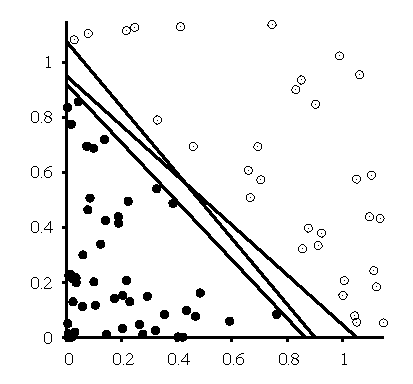
\includegraphics[width=0.4\textwidth]{resources/svm_russel_classification_a}}
        \hspace{0.2cm}
    %TODO:(b) The maximum margin separator (heavy line), is at the midpoint of the margin (area between dashed lines). The support vectors (points with large circles) are the examples closest to the separator.
    \subfloat[O separador com maior margem (linha escura) no ponto médio da margem (entre as linhas pontilhadas). Os vetores de suporte (pontos circulados) são os mais próximos ao separador. \label{fig:svm_classification_b}]
        {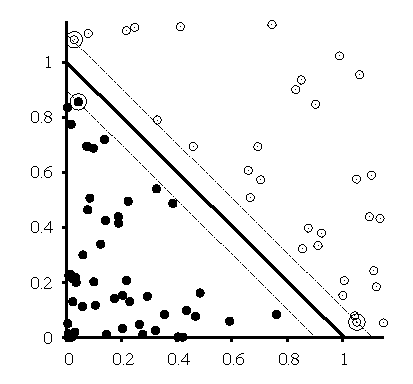
\includegraphics[width=0.4\textwidth]{resources/svm_russel_classification_b}}
        \legend{Fonte: \citeonline[p. 745]{russell:2010}}
\end{figure}
%\textcolor{red}{Testes figura~\ref{fig:svm_classification}, e as figuras~\ref{fig:svm_classification_a}~e~\ref{fig:svm_classification_b}.}


\section{Modelos Formais para Validação de Sistemas}
\label{sec:modelosformais}
Sistemas embarcados são muitas vezes usados em situações críticas, em que segurança e confiabilidade são critérios muito importantes. O uso de modelos formais para descrever o comportamento do sistema antes que este seja desenvolvido é uma forma de se aproximar da melhor confiabilidade, pois esses modelos podem ser validados automaticamente \cite{edwards:1997}.

\subsection{Máquinas de Estado Finitas}
Uma Máquina de Estado Finita (FSM) se baseia em um conjunto finito de estados, entradas, saídas e transições entre estados. A descrição do comportamento baseado em estados é importante na modelagem de sistemas embarcados \cite{marwedel:2010}.

\begin{figure}[h]
	\caption{\label{fig:fsm}Exemplo de diagrama de estados}
	\begin{center}
	    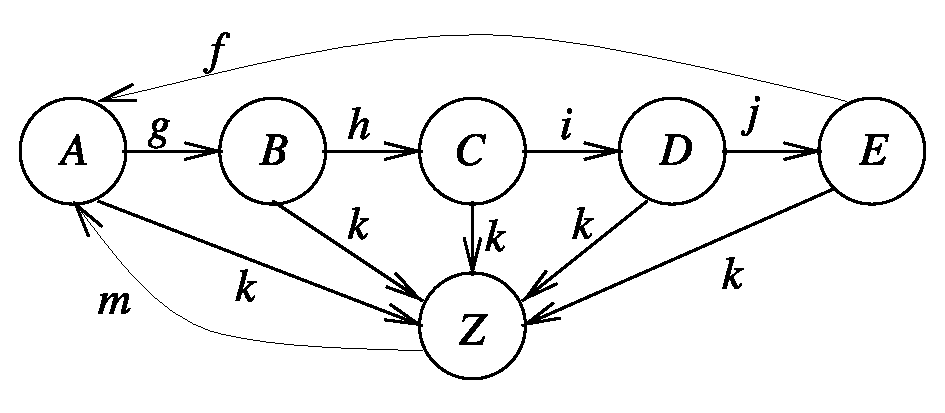
\includegraphics[width=0.5\textwidth]{resources/fsm_marwedel}
	\end{center}
	\legend{Fonte: \citeonline[p. 39]{marwedel:2010}}
\end{figure}

Um diagrama de estados como o da figura~\ref{fig:fsm} é uma representação clássica de uma FSM. Os círculos representam estados, as arestas são transições e o rótulo das arestas são eventos de transição, que levam a máquina a mudar de estado \cite{marwedel:2010}.

\subsection{Redes de Petri}
Uma rede de Petri é um modelo matemático de um sistema, cujo estudo pode revelar informações vitais sobre a estrutura e o comportamento do sistema modelado \cite{peterson:1981}. Segundo \citeonline{murata:1989}, as redes de Petri são uma ferramenta de modelagem matemática e gráfica, especialmente úteis para sistemas concorrentes, assíncronos, distribuídos, paralelos, não-determinísticos, e estocásticos.

A estrutura de uma rede de Petri consiste em lugares, transições, funções de entrada e funções de saída. Graficamente, sua representação é dada por um grafo direcionado, em que os lugares são representados por círculos, as transições por barras, e os arcos entre os lugares e as transições indicam entradas e saídas \cite{peterson:1981}. % $C = (P,T,I,O)

Além disso, cada um dos lugares é marcado com um número não negativo de \textit{tokens}. Quando os lugares têm um número positivo $k$ de \textit{tokens}, estes são representados graficamente por $k$ círculos preenchidos posicionados no interior dos círculos que representam os lugares \cite{murata:1989}, como pode ser visto nos lugares $P_1$ e $P_2$ da figura~\ref{fig:petrinet}. Uma transição é disparada de acordo com um evento determinado, desde que hajam \textit{tokens} suficientes no lugar de entrada.

\begin{figure}[h]
	\caption{\label{fig:petrinet}Exemplo de rede de Petri com atividades paralelas}
	\begin{center}
	    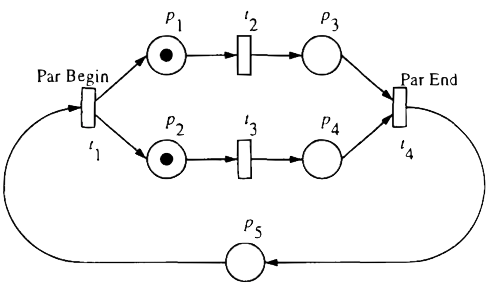
\includegraphics[width=0.5\textwidth]{resources/petri_net_murata_1}
	\end{center}
	\legend{Fonte: \citeonline[p. 545]{murata:1989}}
\end{figure}

Na figura~\ref{fig:petrinet} as transições $t_1$ e $t_2$ estão habilitadas, pois há \textit{tokens} suficientes nos lugares $P_1$ e $P_2$, e também são paralelas, pois suas causas são independentes. Caso uma dessas transições seja disparada, o \textit{token} no lugar de entrada é removido e um novo é produzido no lugar de saída da transição.

\section{Modelagem de software}
\label{sec:modelagem}
\subsection{Transformações de modelo para código}